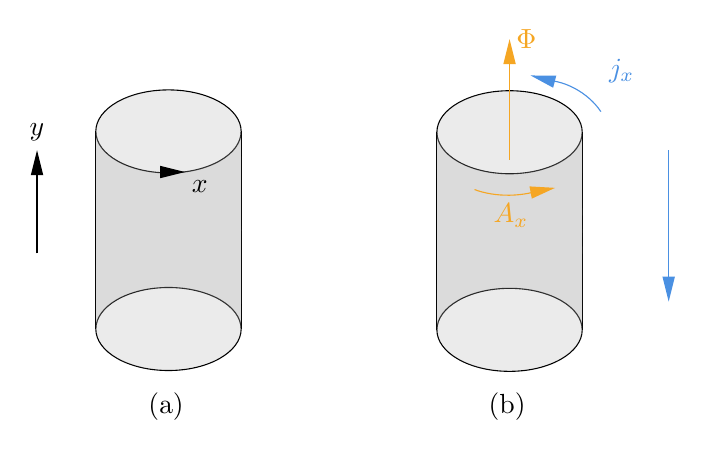
\begin{tikzpicture}[x=0.75pt,y=0.75pt,yscale=-1,xscale=1]
    %uncomment if require: \path (0,300); %set diagram left start at 0, and has height of 300
    
    %Shape: Ellipse [id:dp7184485231494095] 
    \draw   (90,61) .. controls (90,49.95) and (105.67,41) .. (125,41) .. controls (144.33,41) and (160,49.95) .. (160,61) .. controls (160,72.05) and (144.33,81) .. (125,81) .. controls (105.67,81) and (90,72.05) .. (90,61) -- cycle ;
    %Straight Lines [id:da7997452358100254] 
    \draw    (90,61) -- (90,156.19) ;
    %Straight Lines [id:da20276687390866277] 
    \draw    (160,61) -- (160,156.19) ;
    %Shape: Ellipse [id:dp22295770352968924] 
    \draw   (90,156.19) .. controls (90,145.14) and (105.67,136.19) .. (125,136.19) .. controls (144.33,136.19) and (160,145.14) .. (160,156.19) .. controls (160,167.23) and (144.33,176.19) .. (125,176.19) .. controls (105.67,176.19) and (90,167.23) .. (90,156.19) -- cycle ;
    %Shape: Polygon Curved [id:ds25068626323011634] 
    \draw  [draw opacity=0][fill={rgb, 255:red, 155; green, 155; blue, 155 }  ,fill opacity=0.2 ] (90,61) .. controls (92.83,87.74) and (156.83,87.41) .. (160,61) .. controls (160.5,155.11) and (159.5,65.44) .. (160,156.19) .. controls (158.17,180.44) and (94.83,184.44) .. (90,156.19) .. controls (90.17,77.74) and (90.17,156.08) .. (90,61) -- cycle ;
    %Shape: Polygon Curved [id:ds012936936567447432] 
    \draw  [draw opacity=0][fill={rgb, 255:red, 155; green, 155; blue, 155 }  ,fill opacity=0.2 ] (90,156.19) .. controls (92.83,129.44) and (156.83,129.78) .. (160,156.19) .. controls (160.5,62.08) and (159.5,151.75) .. (160,61) .. controls (158.17,36.75) and (94.83,32.75) .. (90,61) .. controls (90.17,139.44) and (90.17,61.11) .. (90,156.19) -- cycle ;
    %Straight Lines [id:da2777301896933302] 
    \draw    (123.17,80.56) -- (131,80.56) ;
    \draw [shift={(133,80.56)}, rotate = 180] [fill={rgb, 255:red, 0; green, 0; blue, 0 }  ][line width=0.08]  [draw opacity=0] (12,-3) -- (0,0) -- (12,3) -- cycle    ;
    %Straight Lines [id:da4704864907693176] 
    \draw    (61.67,119.7) -- (61.67,72.03) ;
    \draw [shift={(61.67,70.03)}, rotate = 90] [fill={rgb, 255:red, 0; green, 0; blue, 0 }  ][line width=0.08]  [draw opacity=0] (12,-3) -- (0,0) -- (12,3) -- cycle    ;
    %Shape: Ellipse [id:dp32276627043311756] 
    \draw   (254.33,61.4) .. controls (254.33,50.35) and (270,41.4) .. (289.33,41.4) .. controls (308.66,41.4) and (324.33,50.35) .. (324.33,61.4) .. controls (324.33,72.45) and (308.66,81.4) .. (289.33,81.4) .. controls (270,81.4) and (254.33,72.45) .. (254.33,61.4) -- cycle ;
    %Straight Lines [id:da2493741248712169] 
    \draw    (254.33,61.4) -- (254.33,156.59) ;
    %Straight Lines [id:da01907222419669452] 
    \draw    (324.33,61.4) -- (324.33,156.59) ;
    %Shape: Ellipse [id:dp8687100286275256] 
    \draw   (254.33,156.59) .. controls (254.33,145.54) and (270,136.59) .. (289.33,136.59) .. controls (308.66,136.59) and (324.33,145.54) .. (324.33,156.59) .. controls (324.33,167.63) and (308.66,176.59) .. (289.33,176.59) .. controls (270,176.59) and (254.33,167.63) .. (254.33,156.59) -- cycle ;
    %Shape: Polygon Curved [id:ds702995349401595] 
    \draw  [draw opacity=0][fill={rgb, 255:red, 155; green, 155; blue, 155 }  ,fill opacity=0.2 ] (254.33,61.4) .. controls (257.17,88.14) and (321.17,87.81) .. (324.33,61.4) .. controls (324.83,155.51) and (323.83,65.84) .. (324.33,156.59) .. controls (322.5,180.84) and (259.17,184.84) .. (254.33,156.59) .. controls (254.5,78.14) and (254.5,156.48) .. (254.33,61.4) -- cycle ;
    %Shape: Polygon Curved [id:ds590026256918492] 
    \draw  [draw opacity=0][fill={rgb, 255:red, 155; green, 155; blue, 155 }  ,fill opacity=0.2 ] (254.33,156.59) .. controls (257.17,129.84) and (321.17,130.18) .. (324.33,156.59) .. controls (324.83,62.48) and (323.83,152.15) .. (324.33,61.4) .. controls (322.5,37.15) and (259.17,33.15) .. (254.33,61.4) .. controls (254.5,139.84) and (254.5,61.51) .. (254.33,156.59) -- cycle ;
    %Shape: Arc [id:dp9125639474648126] 
    \draw  [draw opacity=0] (305.98,88.63) .. controls (301.28,90.49) and (295.62,91.62) .. (289.52,91.73) .. controls (283.19,91.84) and (277.31,90.83) .. (272.44,89.01) -- (289.22,74.7) -- cycle ; \draw  [color={rgb, 255:red, 245; green, 166; blue, 35 }  ,draw opacity=1 ] (305.98,88.63) .. controls (301.28,90.49) and (295.62,91.62) .. (289.52,91.73) .. controls (283.19,91.84) and (277.31,90.83) .. (272.44,89.01) ;  
    %Straight Lines [id:da9836416282060478] 
    \draw [color={rgb, 255:red, 245; green, 166; blue, 35 }  ,draw opacity=1 ]   (302.28,89.9) -- (309.31,88.56) ;
    \draw [shift={(311.28,88.19)}, rotate = 169.23] [fill={rgb, 255:red, 245; green, 166; blue, 35 }  ,fill opacity=1 ][line width=0.08]  [draw opacity=0] (12,-3) -- (0,0) -- (12,3) -- cycle    ;
    
    %Straight Lines [id:da808792480104837] 
    \draw [color={rgb, 255:red, 245; green, 166; blue, 35 }  ,draw opacity=1 ]   (289.33,74.7) -- (289.33,18.57) ;
    \draw [shift={(289.33,16.57)}, rotate = 90] [fill={rgb, 255:red, 245; green, 166; blue, 35 }  ,fill opacity=1 ][line width=0.08]  [draw opacity=0] (12,-3) -- (0,0) -- (12,3) -- cycle    ;
    %Shape: Arc [id:dp527662455456241] 
    \draw  [draw opacity=0] (305,36.37) .. controls (309.73,36.13) and (315.14,37.34) .. (320.45,40.12) .. controls (325.93,42.99) and (330.39,47.06) .. (333.33,51.47) -- (314.04,56.31) -- cycle ; \draw  [color={rgb, 255:red, 74; green, 144; blue, 226 }  ,draw opacity=1 ] (305,36.37) .. controls (309.73,36.13) and (315.14,37.34) .. (320.45,40.12) .. controls (325.93,42.99) and (330.39,47.06) .. (333.33,51.47) ;  
    %Straight Lines [id:da7698889686411401] 
    \draw [color={rgb, 255:red, 74; green, 144; blue, 226 }  ,draw opacity=1 ]   (310.04,36.77) -- (301.4,34.54) ;
    \draw [shift={(299.47,34.04)}, rotate = 14.5] [fill={rgb, 255:red, 74; green, 144; blue, 226 }  ,fill opacity=1 ][line width=0.08]  [draw opacity=0] (12,-3) -- (0,0) -- (12,3) -- cycle    ;
    %Straight Lines [id:da815784149832661] 
    \draw [color={rgb, 255:red, 74; green, 144; blue, 226 }  ,draw opacity=1 ]   (366,70.19) -- (366,141) ;
    \draw [shift={(366,143)}, rotate = 270] [fill={rgb, 255:red, 74; green, 144; blue, 226 }  ,fill opacity=1 ][line width=0.08]  [draw opacity=0] (12,-3) -- (0,0) -- (12,3) -- cycle    ;
    
    % Text Node
    \draw (135,83.56) node [anchor=north west][inner sep=0.75pt]    {$x$};
    % Text Node
    \draw (61.67,67.03) node [anchor=south] [inner sep=0.75pt]    {$y$};
    % Text Node
    \draw (290.01,94.74) node [anchor=north] [inner sep=0.75pt]  [color={rgb, 255:red, 245; green, 166; blue, 35 }  ,opacity=1 ]  {$A_{x}$};
    % Text Node
    \draw (291.33,16.57) node [anchor=west] [inner sep=0.75pt]  [color={rgb, 255:red, 245; green, 166; blue, 35 }  ,opacity=1 ]  {$\Phi $};
    % Text Node
    \draw (336,25) node [anchor=north west][inner sep=0.75pt]  [color={rgb, 255:red, 74; green, 144; blue, 226 }  ,opacity=1 ]  {$j_{x}$};
    % Text Node
    \draw (114,185.5) node [anchor=north west][inner sep=0.75pt]   [align=left] {(a)};
    % Text Node
    \draw (278,185.5) node [anchor=north west][inner sep=0.75pt]   [align=left] {(b)};
    
    
    \end{tikzpicture}
    